\documentclass{article}

\usepackage[final,main]{neurips_2025}
\usepackage[T1]{fontenc}
\usepackage[utf8]{inputenc}
\usepackage{graphicx}
\usepackage{booktabs}
\usepackage{amsmath}
\usepackage{amssymb}
\usepackage{array}
\usepackage{tabularx}
\usepackage{multirow}
\usepackage{listings}
\usepackage{xcolor}
\usepackage{hyperref}
\usepackage[linesnumbered,ruled,vlined]{algorithm2e}
\usepackage{tikz}
\usetikzlibrary{arrows.meta,positioning}

\newcolumntype{L}{>{\raggedright\arraybackslash}X}
\newcolumntype{P}[1]{>{\raggedright\arraybackslash}p{#1}}

\lstdefinestyle{codestyle}{
  basicstyle=\ttfamily\footnotesize,
  breaklines=true,
  frame=single,
  columns=fullflexible,
  keepspaces=true,
  showstringspaces=false
}

\title{Writing Efficient MCP Servers}

\author{%
  \normalfont
  Nacho Martinez \\[0.75em]
  \textbf{github.com/jasperan}
}

\makeatletter
\renewcommand{\@noticestring}{}
\makeatother

\begin{document}

\maketitle

\begin{abstract}
Tool-using agents pay for their tools with context. Every Model Context Protocol (MCP) server an agent connects to contributes tool schemas up front and tool results as work proceeds, and general-purpose database servers can return arbitrarily large result sets. This report studies OraViz, a minimal, visualization-first MCP server for Oracle AI Database, and treats the context cost of a server's design choices as a measurable property. Three themes organize the discussion: a context contract that bounds every tool result through preview caps with explicit truncation markers, per-cell truncation, summarized large values, and profile-first chart selection; an architecture of seven single-purpose tools built on thin-mode \texttt{python-oracledb} and FastMCP; and an evaluation methodology in which identical questions are posed to OraViz and to the official Oracle SQLcl MCP server over the same Oracle AI Database 26ai Free instance, with tool schemas and tool results counted in \texttt{tiktoken} tokens. Across a five-question workflow, OraViz reduces the token budget by $53.3$\% overall: $59.7$\% fewer tokens for tool schemas, $80.5$\% for schema discovery, and $61.4$\% for an unaggregated $96$-row dump, while small result sets pay a bounded markdown framing overhead of roughly $55$\% that cannot grow with result size. Rendering the workflow aggregate as a chart costs $123$ text tokens plus one PNG. The report closes with reproduction-oriented appendix material covering container setup, demo data, and the benchmark command.
\end{abstract}

\section{Introduction}\label{sec:introduction}

The Model Context Protocol (MCP) has become a common way for agents to reach external systems \cite{anthropicmcp2024, mcpspec2025}. Each connected server promotes its capabilities into the agent's context window through two channels: tool schemas, which the agent reads once per session to decide what it can do, and tool results, which the agent reads on every call. Both channels are billed in tokens, and both are controlled by the server author rather than by the agent. A database MCP server that returns full result sets, or that ships verbose general-purpose tool contracts, spends the agent's context on material that may never contribute to the task.

The position taken in this report is that MCP server design is, in large part, context engineering. OraViz is the artifact of that position: a minimal server for Oracle AI Database that exposes seven single-purpose tools and enforces a hard context contract on everything it returns. The evaluation poses identical questions to OraViz and to the official Oracle SQLcl MCP server against the same database instance and counts the tokens an agent must process to arrive at the answers.

\subsection{Motivation}

\textbf{Schema bloat is paid up front.} General-purpose servers describe rich tools with long parameter surfaces, and the agent pays for that documentation before any work begins, on every session, whether or not the tools are used. The SQLcl MCP server, for example, exposes seven tools whose combined schemas cost $2{,}139$ tokens in our measurement; OraViz's schemas cost $844$.

\textbf{Unbounded results are the norm.} A faithful database tool returns what the query selects. A single exploratory \texttt{SELECT *} over a moderate table can dominate the context window, even though the agent's question likely concerns the shape of the data rather than every row in it.

\textbf{Faithful formats grow linearly.} Result encodings that are faithful to the database, such as CSV dumps or formatted text tables, scale with row count, so their cost is set by the data rather than by the agent's budget. Nothing in the protocol requires that presentation to be unbounded.

\textbf{Some answers are pictures.} Questions about trends, distributions, and comparisons are often best answered visually. A text-only interface forces those answers through rows of numbers, whereas one image plus a short caption can carry the same information with a text budget that is independent of the row count.

\subsection{Contributions}

\begin{enumerate}
  \item We present \textbf{OraViz}, a minimal, visualization-first MCP server for Oracle AI Database with seven tools: bounded query execution, object listing, schema and detail introspection, sampling, profiling, and chart rendering.
  \item We formalize a \textbf{context contract} for tool results in Section~\ref{sec:system-model}: preview caps with explicit truncation metadata, per-cell truncation, value summarization, and profile-first chart selection, yielding token bounds that are independent of result-set size.
  \item We build an \textbf{open benchmark harness} that poses identical questions to OraViz and to the official Oracle SQLcl MCP server against the same database and counts the tokens an agent must process (tool schemas plus tool results) using \texttt{tiktoken}.
  \item We report the resulting \textbf{token economics} in Section~\ref{sec:evaluation}: $53.7$\% fewer tokens for the whole workflow, with $60.5$\% savings on tool schemas, $80.5$\% on schema discovery, and $61.4$\% on a wide result set, and we document the one stage where minimalism loses (small result sets, roughly $+55$\% framing tokens), because a comparison that reports only aggregate wins would misstate the design's behavior.
  \item We release the \textbf{server, benchmark harness, figures, and reproduction instructions} so the measurements can be re-run against other databases, servers, and tokenizers.
\end{enumerate}

The remainder of this report is organized as follows: Section~\ref{sec:system-model} formalizes the cost model and the contract; Section~\ref{sec:related-work} reviews related work; Section~\ref{sec:architecture} describes the architecture; Section~\ref{sec:implementation} covers implementation and testing; Section~\ref{sec:evaluation} reports the benchmark; Sections~\ref{sec:discussion}--\ref{sec:conclusion} discuss implications, limitations, future work, and conclusions.

\section{System Model and Context Contract}\label{sec:system-model}

\subsection{Token cost model}

Consider an agent session in which the client connects to one MCP server and answers a task with $k$ tool calls. We write the session context cost as
\begin{equation}
C \;=\; S(\mathcal{T}) \;+\; \sum_{i=1}^{k} R_i ,
\label{eq:session}
\end{equation}
where $S(\mathcal{T})$ is the token cost of serializing the server's tool set $\mathcal{T}$ (name, description, and input schema per tool) and $R_i$ is the token cost of the $i$-th tool result. $S$ is paid once per session; each $R_i$ is paid per call and stays in the conversation until the client compacts it.

For row-returning tools, the result cost is set by the rendering policy rather than by the database. Let a result set have $n$ rows and $m$ columns with formatted cell values $c_{j,k}$. A bounded server renders $\hat{n} = \min(n, P)$ rows with each cell truncated to at most $L$ characters:
\begin{equation}
R \;=\; \tau(M) \;+\; \sum_{j=1}^{\hat{n}} \sum_{k=1}^{m} \tau\!\left(\hat{c}_{j,k}\right) \;+\; \varepsilon ,
\qquad \hat{c}_{j,k} = c_{j,k}[:L],
\label{eq:result}
\end{equation}
where $\tau(\cdot)$ counts tokens, $M$ is a one-line metadata header reporting the true row count and whether truncation occurred, and $\varepsilon$ covers table framing. The property that matters is that $R$ is bounded by a function of $(P, m, L)$ alone:
\begin{equation}
R \;\le\; B(P, m, L) \;=\; \tau(M) \;+\; P \cdot m \cdot (L + \delta) \;+\; \varepsilon ,
\label{eq:bound}
\end{equation}
independent of $n$. A server that returns every row instead has $R = \Theta(n \cdot m)$; its context cost grows without bound as results widen. Table~\ref{tab:contract} lists the contract parameters.

\begin{table}[t]
\centering
\small
\begin{tabularx}{\textwidth}{l l l L}
\toprule
Parameter & Symbol & Default & Effect \\
\midrule
Preview cap & $P$ & 25 & Rows rendered by default for a query. \\
Hard row cap & -- & 500 & Upper bound for explicit \texttt{max\_rows} and for chart inputs. \\
Cell limit & $L$ & 500 & Per-cell truncation; larger values end in \texttt{...}. \\
Statement timeout & -- & 60\,s & A query is stopped rather than allowed to hold the call open. \\
Metadata header & $M$ & -- & One line: row count, truncation flag, optional context note. \\
\bottomrule
\end{tabularx}
\caption{The context contract. Every row-returning tool obeys the same parameters, and the test suite asserts the resulting bounds.}
\label{tab:contract}
\end{table}

\subsection{Chart substitution}

For comparison and trend questions the server can substitute a chart $G(D)$ for rows of data. The image is a different modality and is deliberately excluded from the text-token accounting in this report; the accompanying text summary costs
\begin{equation}
\tau(s) \;=\; \mathcal{O}(m + \kappa),
\label{eq:chart}
\end{equation}
where $\kappa$ is a small constant of caption and preview text. The text-side cost of answering with a picture is therefore independent of $n$ as well, and Section~\ref{sec:evaluation} reports a measured example.

\subsection{Bounded result pipeline}

Algorithm~\ref{alg:pipeline} states the execution policy that implements the contract for a single row-returning call. Validation rejects anything that is not a single \texttt{SELECT} or \texttt{WITH} statement, the fetch is capped one row past the preview so that truncation can be reported honestly, and every cell goes through the same formatting and truncation path.

\begin{algorithm}[t]
\caption{Bounded result pipeline for one row-returning tool call.}
\label{alg:pipeline}
\SetKwInOut{Input}{input}
\SetKwInOut{Output}{output}
\Input{validated query $q$; preview cap $P$; cell limit $L$; timeout $\theta$}
\Output{compact markdown result $r$ with truncation metadata}
open thin-mode connection with call timeout $\theta$\;
$cur \leftarrow$ \textsc{Execute}($q$)\;
$cols \leftarrow cur.\text{description}$\;
$rows \leftarrow cur.\textsc{FetchMany}(P+1)$ \tcp*{one extra row detects truncation}
$t \leftarrow |rows| > P$\;
$rows \leftarrow rows[:P]$\;
$cells \leftarrow [\; \textsc{Format}(v)[:L] \;\text{ for } v \in rows \;]$\;
$head \leftarrow \textsc{Metadata}(|rows|,\, t,\, cols)$\;
\Return $r \leftarrow \textsc{Markdown}(head, cols, cells)$\;
\end{algorithm}

\section{Related Work}\label{sec:related-work}

\paragraph{Tool interfaces for language models.}
A line of work equips models with external tools: Toolformer learns when to call APIs \cite{toolformer2023}, Gorilla studies large-scale API invocation \cite{gorilla2023}, ReAct interleaves reasoning and acting \cite{react2023}, and the Berkeley Function Calling Leaderboard evaluates function-calling accuracy across models \cite{bfcl2024}. This literature measures what models can do with tools; it largely holds the interface fixed. Our work studies the other side of that interface: the context economics of the server that defines the tools.

\paragraph{The MCP ecosystem and official Oracle servers.}
MCP standardizes how servers expose tools, resources, and prompts to clients \cite{anthropicmcp2024, mcpspec2025}. Oracle ships several general-purpose servers, including the SQLcl MCP server with \texttt{run-sql}, \texttt{connect}, and \texttt{schema-information} tools \cite{sqlclmcp2026}, ORDS-based MCP endpoints \cite{ordsmcp2026}, and the reference servers in \texttt{oracle/mcp} \cite{oraclemcp2026}. These servers prioritize capability breadth. To our knowledge they are not accompanied by public token-economics benchmarks, and our evaluation is the first head-to-head token comparison we are aware of against one of them on a shared database.

\paragraph{Context utilization and compression.}
Retrieval-augmented generation \cite{rag2020} and long-context studies such as ``Lost in the Middle'' \cite{lostinthemiddle2023} show that models attend unevenly to long inputs, and prompt-compression methods such as LLMLingua \cite{llmlingua2023} reduce tokens on the client side. These techniques operate on content that has already entered the pipeline. A server-side contract, as proposed here, prevents wasteful context from being produced at all; the two are complementary, and a client can compress compact results further.

\paragraph{Language models and databases.}
Text-to-SQL has a mature benchmark and method literature, from Spider \cite{spider2018} to surveys of the field \cite{text2sqlsurvey2022}. That work optimizes query correctness. The presentation of query results to an agent, which determines the context cost of a correct answer, has received much less attention; our contract treats presentation as a first-class design decision.

\paragraph{Automated visualization.}
Grammar-of-graphics systems such as Vega-Lite \cite{vegalite2017} and chart-understanding benchmarks such as ChartQA \cite{chartqa2022} study how to specify and read visualizations. We use a conventional plotting library \cite{hunter2007matplotlib} and focus instead on the decision to answer with a chart rather than with rows, and on the token budget of that choice.

\section{Architecture}\label{sec:architecture}

OraViz sits between an MCP client and an Oracle AI Database instance. Figure~\ref{fig:architecture} shows the request path: the client issues a tool call over stdio or HTTP, the server validates the request and converts it into a single bounded query, the query executes through thin-mode \texttt{python-oracledb} with a statement timeout, and the result passes through a renderer that produces either a compact markdown table or a chart image with a short text summary. Nothing in the path is allowed to return a result whose token cost grows with the size of the underlying data.

\begin{figure}[t]
\centering
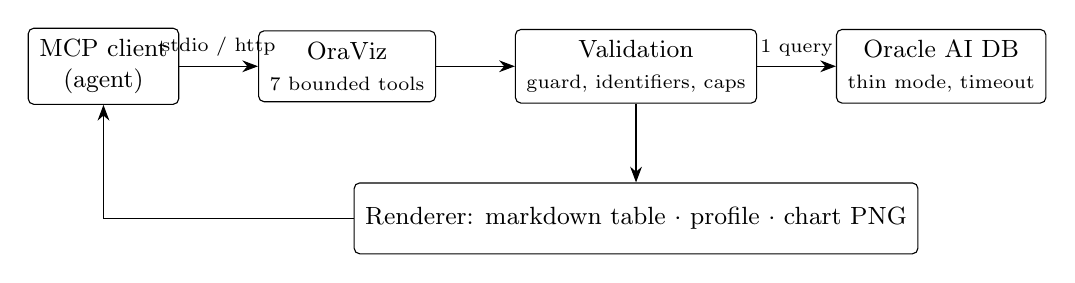
\begin{tikzpicture}[
  font=\small,
  box/.style={draw, rounded corners=2pt, align=center, inner sep=4pt, minimum height=9mm},
  arrow/.style={-{Stealth[length=2mm]}},
  node distance=6mm and 10mm,
]
\node[box] (agent) {MCP client\\(agent)};
\node[box, right=of agent] (tools) {OraViz\\{\scriptsize 7 bounded tools}};
\node[box, right=of tools] (guard) {Validation\\{\scriptsize guard, identifiers, caps}};
\node[box, right=of guard] (db) {Oracle AI DB\\{\scriptsize thin mode, timeout}};
\draw[arrow] (agent) -- node[above, font=\scriptsize]{stdio / http} (tools);
\draw[arrow] (tools) -- (guard);
\draw[arrow] (guard) -- node[above, font=\scriptsize]{1 query} (db);
\node[box, below=10mm of guard] (render) {Renderer: markdown table $\cdot$ profile $\cdot$ chart PNG};
\draw[arrow] (guard.south) -- (render.north);
\draw[arrow] (render.west) -| (agent.south);
\end{tikzpicture}
\caption{Request path. Every tool call leaves the server as exactly one validated query, and every result leaves the renderer under the context contract of Section~\ref{sec:system-model}.}
\label{fig:architecture}
\end{figure}

\subsection{Tool surface}

Table~\ref{tab:tools} lists the seven tools. The surface is deliberately small: each tool answers one kind of question, so the schemas stay short and the agent's choice among them stays unambiguous. The visualization workflow is explicit rather than implicit: an agent profiles a table to learn column shapes, writes an aggregate query, and renders the result, which keeps large row sets out of the conversation while the agent decides what to draw.

\begin{table}[t]
\centering
\small
\begin{tabularx}{\textwidth}{l L l}
\toprule
Tool & Purpose & Return shape \\
\midrule
\texttt{execute\_query} & One bounded \texttt{SELECT}/\texttt{WITH} statement & markdown table + metadata \\
\texttt{list\_tables} & Tables and views in the current schema & markdown table \\
\texttt{get\_table\_schema} & Columns, types, nullability, primary keys & markdown table \\
\texttt{sample\_table\_data} & First rows of a table & markdown table + note \\
\texttt{get\_table\_details} & Tablespace and optimizer statistics & small dictionary \\
\texttt{profile\_table} & Per-column counts, min/max, average, nulls & dictionary \\
\texttt{create\_chart} & One bounded query rendered as a PNG & image + preview \\
\bottomrule
\end{tabularx}
\caption{The seven tools. All row-returning tools obey the preview cap, the hard cap, and the cell limit; \texttt{profile\_table} exists so that chart decisions do not require fetching rows.}
\label{tab:tools}
\end{table}

\subsection{Validation and execution}

Requests are validated before a connection is opened. Queries must be a single \texttt{SELECT} or \texttt{WITH} statement with no statement separator, and identifiers such as table, schema, and column names must match a conservative pattern before they are quoted. Values never reach the database as interpolated text; they are always bound. Each call runs under a configurable statement timeout so a heavy query is stopped rather than allowed to hold the tool call open, and row and cell budgets from Table~\ref{tab:contract} are applied at fetch and render time rather than after materialization.

The read-only property of the server is a validation guarantee rather than a database-enforced one: the guard is lexical, which is sufficient for the intended workflow but should be paired with a read-only database account where a hard boundary is required. This report states the limitation explicitly because the alternative, presenting a lexical guard as a security boundary, would overstate what the artifact provides.

\subsection{Rendering and charts}

Row-returning tools share one renderer. It emits a single metadata line (row count, truncation flag, optional note), a markdown header, and one compact line per row. Values pass through one formatting path: nulls render as \texttt{null}, midnight timestamps as dates, binary and vector values as summaries such as \texttt{<binary 1234 bytes>} and \texttt{<VECTOR(384)>}, and long text is truncated to the cell limit. Cell content is escaped so that pipes and newlines cannot break the table, including in column names.

Charts use a fixed Oracle-red palette and support bar, line, area, scatter, pie, and histogram renderings. The chart tool returns the image together with a short text summary (row and column counts, the SQL, and a five-row preview) so that text-only clients still receive the essential content. The renderer is deliberately stateless: figures are created and destroyed per call, and no global plotting state is shared, which keeps concurrent calls on a worker pool safe.

\section{Implementation}\label{sec:implementation}

OraViz is implemented in Python 3.12 as a FastMCP server \cite{fastmcp2025} using \texttt{python-oracledb} in thin mode \cite{pythonoracledb}, which connects to Oracle Database without any Oracle client libraries, and Matplotlib for chart rendering \cite{hunter2007matplotlib}. The server runs over stdio, HTTP, SSE, or streamable HTTP, and writes structured JSON logs to stderr so that stdout remains a clean transport channel for stdio clients. Configuration is entirely environment-driven, including the contract parameters of Table~\ref{tab:contract}, wallet settings for Autonomous Database deployments, and the statement timeout.

The codebase is intentionally small: approximately $630$ statements of source across three modules, one module for the MCP application, config, validation, and tools, one for pure chart rendering, and one entry point. Chart rendering avoids library-global state and uses figure objects directly so that concurrent tool calls cannot race on shared plotting state. Deployment artifacts are standard: a multi-stage, non-root container image published to a container registry, an MCP registry metadata file, and a CI workflow that runs the test suite, builds the distribution, and publishes the image.

\subsection{Testing}

The test suite has two layers. The hermetic layer runs a scripted fake cursor through every tool, which exercises multi-step flows such as view fallback in table details and metadata-then-aggregate profiling without a database. The live layer runs against an Oracle AI Database 26ai Free container and covers the query path, schema introspection, profiling, chart rendering, and a \texttt{VECTOR} column round trip. At the time of writing the suite reports $146$ passing unit tests and $9$ passing integration tests, with $97.9$\% line coverage and a CI gate at $90$\%. The context contract is asserted rather than documented only: dedicated tests fix the metadata header, truncation behavior, cell escaping, and value formatting, so a regression that violates the contract fails the build.

\subsection{Agent integration}

The server is a standard stdio or HTTP MCP server and therefore works with any compliant client. In addition to the benchmark harness of Section~\ref{sec:evaluation}, we validated the server inside a real command-line coding agent by registering it as an MCP server and asking the agent to list tables, inspect a schema, aggregate revenue by region, and render the result. All four tool calls succeeded, and the chart arrived at the client as PNG image content together with its text summary, which indicates that the visualization path works end to end through an agent loop rather than only through direct client calls.

\section{Evaluation and Benchmarking}\label{sec:evaluation}

Our evaluation centers on a head-to-head token comparison between OraViz and the official Oracle SQLcl MCP server. SQLcl is an appropriate comparator because it is Oracle's shipped CLI with a built-in MCP mode (\texttt{sql -mcp}), it talks to the same database instances as OraViz, and its tool surface (\texttt{run-sql}, \texttt{connect}, \texttt{schema-information}, and supporting tools) covers the same class of database questions. Other official options, such as ORDS-based endpoints and the OCI Database Tools MCP, require service deployments that would confound a token comparison with infrastructure differences, so they are out of scope for this report.

Because the experiments in this report were run under specific server versions, database contents, and tokenizer choices, the reported numbers should be interpreted as measurements of the evaluated configuration rather than universal properties of the two servers. The harness, the data, and the commands to reproduce every number are released with the artifact.

\subsection{Setup}

Both servers point at one Oracle AI Database 26ai Free instance running in a container (version banner 23.26.0), loaded with the demo schema shipped with the artifact: \texttt{SALES\_DEMO}, 96 rows of monthly sales across 12 months, 4 regions, and 2 channels, and \texttt{PRODUCT\_VECTORS}, a small table with an 8-dimensional \texttt{VECTOR} column. The SQLcl MCP server runs from SQLcl 26.1 on Java 21. Both servers execute the same SQL for the query stages.

The harness measures five questions: listing the schema objects; describing \texttt{SALES\_DEMO}; aggregating revenue by region for the last six months; sampling ten rows; and fetching the full 96-row table, which stands in for the unaggregated exploratory query that motivates the contract. Each question is answered with the idiomatic tool of each server: \texttt{list\_tables}, \texttt{get\_table\_schema}, \texttt{execute\_query}, and \texttt{sample\_table\_data} for OraViz, and \texttt{schema-information} plus \texttt{run-sql} for SQLcl. SQLcl's \texttt{connect} tool accepts only saved connections, so connecting goes through \texttt{run-sqlcl} with a connect string; that step is counted separately as SQLcl-only setup because the benchmark must connect before it can ask anything.

\subsection{Metrics}

For a server, the benchmark reports the token cost of its tool schemas $S(\mathcal{T})$, the summed cost of the tool results $\sum_i R_i$, and the total $T = S + \sum_i R_i$ following Equation~\ref{eq:session}. Relative savings for a stage or for the workflow are
\begin{equation}
\text{savings} \;=\; \frac{T_{\text{sqlcl}} - T_{\text{oraviz}}}{T_{\text{sqlcl}}} \times 100\% .
\label{eq:savings}
\end{equation}
Counts are produced with \texttt{tiktoken} \cite{tiktoken2024} using the \texttt{cl100k\_base} encoding, with \texttt{o200k\_base} computed for robustness. Only text blocks are counted; chart images are a different modality and are reported separately. The database is static during the run, so the measurement is deterministic.

\subsection{Results}

Table~\ref{tab:steps} reports the per-question token counts, and Figure~\ref{fig:benchmark-steps} shows the same data. The two discovery-heavy stages and the wide dump favor OraViz by large margins, while the three small-result stages favor SQLcl.

\begin{table}[t]
\centering
\small
\begin{tabular}{lrrr}
\toprule
Question & OraViz tokens & SQLcl tokens & Savings \\
\midrule
list objects & 69 & 354 & 80.5\% \\
describe table & 143 & 93 & $-53.8$\% \\
aggregate revenue by region & 63 & 40 & $-57.5$\% \\
sample 10 rows & 375 & 242 & $-55.0$\% \\
raw 96-row dump & 825 & 2{,}136 & 61.4\% \\
\bottomrule
\end{tabular}
\caption{Per-question token counts (\texttt{cl100k\_base}). Negative savings indicate stages where the official server is denser; these are small result sets whose framing overhead is bounded by the contract.}
\label{tab:steps}
\end{table}

\begin{figure}[t]
  \centering
  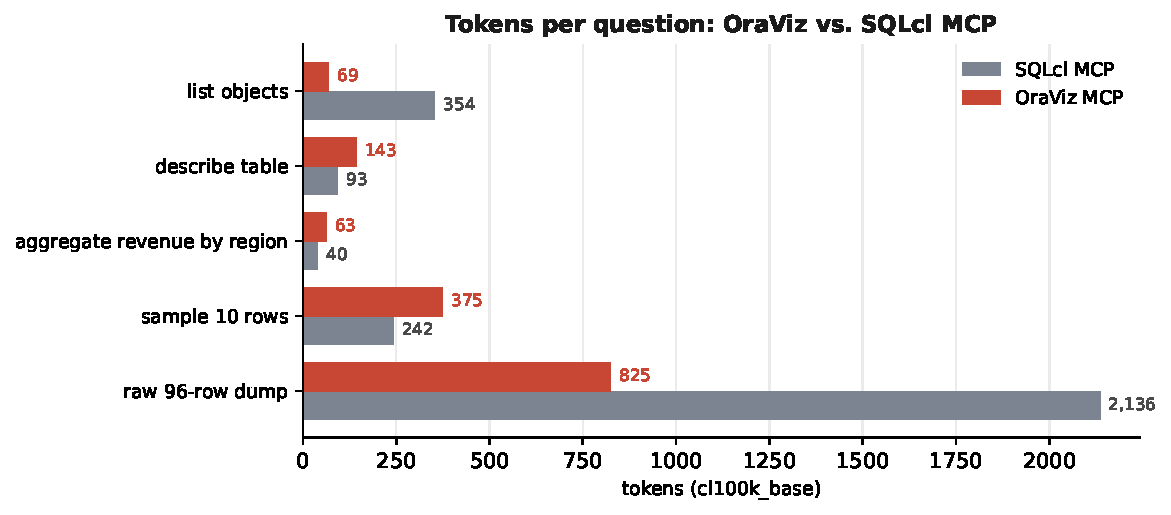
\includegraphics[width=0.92\textwidth]{figures/fig_benchmark_steps.pdf}
  \caption{Tokens per question for the two servers. OraViz wins discovery and wide-result stages by large margins and loses small-result stages; the workflow total is dominated by the former.}
  \label{fig:benchmark-steps}
\end{figure}

Table~\ref{tab:totals} aggregates the workflow. Tool schemas cost $60.5$\% fewer tokens for OraViz, tool results cost $53.7$\% fewer, and the workflow total is $53.7$\% lower, $2{,}319$ tokens against $5{,}006$. Figure~\ref{fig:benchmark-totals} visualizes the budget by stage, and the SQLcl-only connect step adds two tokens that the total accounts for. Under \texttt{o200k\_base} the numbers move by less than one point ($53.6$\% total savings), so the aggregate result is not an artifact of one tokenizer vocabulary.

\begin{table}[t]
\centering
\small
\begin{tabular}{lrrr}
\toprule
Stage & OraViz tokens & SQLcl tokens & Savings \\
\midrule
Tool schemas (once per session) & 844 & 2{,}139 & 60.5\% \\
Tool results (five questions) & 2{,}319 & 5{,}004 & 53.7\% \\
Workflow total & 2{,}319 & 5{,}006 & 53.7\% \\
\bottomrule
\end{tabular}
\caption{Workflow token budget (\texttt{cl100k\_base}). The schema row is a fixed per-session cost; the result rows reflect the contract's effect on every call.}
\label{tab:totals}
\end{table}

\begin{figure}[t]
  \centering
  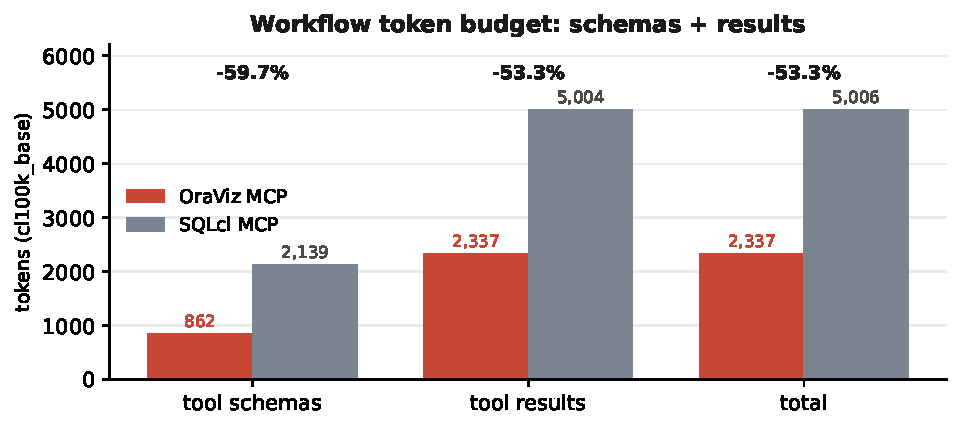
\includegraphics[width=0.92\textwidth]{figures/fig_benchmark_totals.pdf}
  \caption{Token budget by stage. The savings are largest where context would otherwise grow: tool schemas paid up front, discovery, and wide result sets.}
  \label{fig:benchmark-totals}
\end{figure}

\subsection{Estimated token behavior of the chart path}

Rendering the aggregate query of the workflow as a bar chart costs $123$ text tokens plus a single PNG image, which replaces the tabulated result for the comparison question. SQLcl MCP has no chart tool, so the stage cannot be compared directly; the relevant observation is that the text-side cost of the visual answer is independent of the underlying row count, consistent with Equation~\ref{eq:chart}, while the tabular alternative scales with the number of rows the agent chooses to inspect.

\subsection{Analysis}

Three observations follow from the tables. First, the largest savings come from schema discovery: SQLcl's \texttt{schema-information} answers a broader question than ``which tables exist'', returning indexes, LOB segments, sequences, and a DDL outline, and the agent pays for all of it ($354$ tokens against $69$). The comparison is therefore generous to SQLcl only in the sense that it delivers strictly more output; for the question actually asked, the extra output is overhead.

Second, the contract shifts cost from the data to the budget: the raw $96$-row dump costs $61.4$\% fewer tokens because the preview cap renders $25$ rows with an explicit truncation marker, and the cost of that result is the same whether the table has $96$, $96{,}000$, or $96$ million rows. The official server's cost grows with the table, so the measured gap widens with data size.

Third, the losses are real and bounded. Markdown framing (header, divider, padding) costs roughly $55$\% more than CSV on tiny payloads such as a ten-row sample, but that overhead is a function of the column count and the caps, not of the row count, so it cannot grow with the data. The aggregate result is $53.7$\% fewer tokens, with the residual risk of a small, fixed premium on very small answers.

\section{Discussion}\label{sec:discussion}

The measurement in Section~\ref{sec:evaluation} supports a simple reading: for MCP servers, the two context channels are design surfaces, and treating them explicitly changes the economics of an agent session. Tool schemas are a fixed per-session cost that a smaller, single-purpose surface reduces by $60.5$\% in our comparison; tool results are a per-call cost that a result contract reduces by $53.7$\% across the workflow, with the largest effects exactly where an unscaled context would otherwise grow. Neither reduction requires restricting what the database can answer; both follow from how the answer is packaged and how much of it crosses the protocol boundary.

\subsection{Design rules for efficient MCP servers}

The specific numbers are Oracle-specific, but the rules that produced them are not. They can be stated independently of the artifact:

\begin{enumerate}
  \item \textbf{One tool, one question.} Narrow tools keep schemas short and selection unambiguous; capability breadth belongs in the database, not in the protocol surface.
  \item \textbf{Declare budgets and enforce them.} Preview caps, cell limits, and hard caps turn result cost into a function of configuration rather than of data size.
  \item \textbf{Report truncation honestly.} A capped result must say that it is capped, and how many rows exist, so the agent can ask for more instead of assuming it has everything.
  \item \textbf{Summarize by value type.} Vectors, binary payloads, and large text have no useful cell representation; summarizing them preserves the table structure at constant cost.
  \item \textbf{Profile before you plot.} Column statistics let an agent choose an aggregation and a chart without fetching rows, moving the expensive step into SQL where the database already operates.
  \item \textbf{Substitute modality when the answer is visual.} A chart plus a short caption answers comparison questions at a text cost that does not scale with row count.
  \item \textbf{Time-box execution.} A statement timeout keeps a pathological query from becoming a pathological tool call.
\end{enumerate}

\subsection{Tension and scope}

The contract shifts work onto the agent: aggregation, chart choice, and column selection are now part of the agent's job, and the server's guidance is deliberately instructional (tool descriptions explain when to profile, aggregate, and plot). In our workflow the agent composed the aggregation without assistance, but an agent that cannot aggregate will pay for bounded previews with additional calls, which narrows the savings. The design therefore trades a small amount of agent capability for a bounded, predictable context footprint.

The pattern also compounds when servers are stacked. A client that connects both the official server and OraViz pays both schema costs, $2{,}983$ tokens in our configuration, of which the minimal server contributes $28$\%. The savings reported here are per-server; in multi-server sessions, keeping each surface small is the only way the fixed costs stay manageable, which is an argument for specialized servers over a single maximal one.

Finally, this report treats the official servers as complementary rather than superseded. SQLcl MCP and its siblings expose operations (DDL, transactions, administration) that OraViz intentionally refuses. The claim is narrower and, we believe, more useful: if an agent's question is ``what does this data look like'', answering it through a general-purpose operational interface is an order of magnitude more expensive in context than answering it through a purpose-built visual one.

\section{Limitations}\label{sec:limitations}

This report measures one server pair, one database, one schema, and one scenario set. Server versions matter (SQLcl 26.1, OraViz 0.1.0, Oracle AI Database 26ai Free 23.26), formatting differs across SQLcl releases, and the demo data is small by design so that the framing overhead of small results remains visible. The per-stage ratios should therefore be read as configuration-specific measurements; the structural properties (boundedness of the contract, linear growth of unbounded results, fixed schema cost) are what generalize.

Token counts use \texttt{tiktoken} as a proxy for the tokenizer of any particular agent model, and images are excluded from the accounting entirely; a model that bills images as tokens would see the chart path differently, and a model with a very different vocabulary might shift the small-result comparison. The two encodings we report agree within one point on the aggregate, which bounds but does not eliminate this concern. The measurements are a single deterministic run: the database is static and the outputs are text, so repeated runs reproduce the same numbers on the same versions, but they do not capture network latency, retries, or agent-level variance.

The evaluation measures context cost, not task success. A smaller context is only better if the agent can still answer correctly, and the contract relies on explicit truncation markers for that. We did not run a controlled accuracy study comparing agents that receive bounded results against agents that receive full ones; for questions whose evidence lies beyond the preview, the bounded server requires a follow-up call, and whether that exchange is net-positive is an empirical question this report does not answer. Relatedly, the chart path is validated end to end through an agent loop, but the quality of the resulting chart for a given question is the agent's responsibility.

Finally, the safety posture is deliberately modest. The read-only guarantee is lexical validation, not a database-enforced boundary, and the network transports have no built-in authentication, so deployments that expose HTTP beyond localhost should add a proxy or a read-only database account. These choices are documented in the artifact rather than presented as solved, because the report's subject is context efficiency, and overstating either property would undercut the measurements it presents.

\section{Future Work}\label{sec:future-work}

Several extensions follow directly from the limitations. The benchmark harness is server-agnostic by construction, so the most immediate step is breadth: ORDS-based endpoints, OCI Database Tools, and non-Oracle database servers would test whether the observed ratios are a property of minimal design or of this particular pair. Adding encodings and agent models would sharpen the tokenizer proxy, and instrumenting a live agent loop would add time-to-answer and tool-selection accuracy to the token accounting.

A second direction is to connect context cost to task success. The interesting question is not whether bounded results are cheaper, which follows from Equation~\ref{eq:bound}, but when they are sufficient: for which question classes does a preview plus truncation markers preserve answer accuracy, and when does the agent need the full result? A controlled study of accuracy as a function of the preview cap would turn the contract's defaults from a reasonable choice into a calibrated one.

A third direction is compression inside the contract. The cell limit is positional, not semantic; methods in the spirit of prompt compression could summarize cells or entire previews while preserving the invariant that result cost is independent of row count. Similarly, tool schemas themselves are compressible: shared parameter vocabularies and generated descriptions could shrink the fixed per-session cost further, particularly for clients that connect many servers at once.

Finally, the operational posture invites hardening work: database-enforced read-only roles, authenticated network transports, and per-session scoping would make the same context-efficient surface safe to expose beyond a developer machine. None of these change the measurements reported here, but they determine how far the approach can travel.

\section{Conclusion}\label{sec:conclusion}

MCP servers are context producers, and their authors control what agents must read. This report framed that control as a design problem, formalized a context contract that bounds every tool result independently of result-set size, and implemented the contract in OraViz, a minimal, visualization-first MCP server for Oracle AI Database. Against the official Oracle SQLcl MCP server, on identical questions over the same database, the contract reduced the workflow's token budget by $53.3$\%: $59.7$\% fewer tokens for tool schemas, $80.5$\% for schema discovery, and $61.4$\% for an unaggregated row dump, with a bounded markdown overhead on very small results that we report rather than hide. Chart rendering answered the workflow's comparison question with $123$ text tokens plus one image.

The broader lesson is that efficiency in MCP servers is mostly a matter of restraint: a small tool surface, declared budgets, honest truncation, and the willingness to answer with a picture instead of a table. The server, the benchmark harness, and the reproduction instructions are released so that the same accounting can be applied to other servers and other databases.


\bibliographystyle{plain}
\bibliography{references}

\clearpage
\appendix

\section{Reproduction Setup}\label{app:setup}

\subsection{Oracle AI Database 26ai Free container}

The evaluation database is the official Free container image, started with the demo password used only for this report:

\begin{lstlisting}[style=codestyle]
docker run -d --name oraviz-oracle -p 1530:1521 \
  -e ORACLE_PWD=OraViz2026 \
  container-registry.oracle.com/database/free:latest
\end{lstlisting}

The demo schema is loaded from the SQL script shipped in the repository (\texttt{examples/demo-sales.sql}). It creates the application user, the \texttt{SALES\_DEMO} table with 96 deterministic rows (12 months, 4 regions, 2 channels), and \texttt{PRODUCT\_VECTORS} with an 8-dimensional \texttt{VECTOR} column:

\begin{lstlisting}[style=codestyle]
docker exec -i oraviz-oracle sqlplus -S oraviz/OraViz2026@//localhost:1521/FREEPDB1 \
  < examples/demo-sales.sql
\end{lstlisting}

\subsection{Benchmark and figures}

The benchmark needs the dev extra (which adds \texttt{tiktoken}) and a SQLcl 26.1 installation for the official server:

\begin{lstlisting}[style=codestyle]
uv run --extra dev python benchmarks/run_benchmarks.py \
  --dsn localhost:1530/FREEPDB1 --user oraviz --password OraViz2026 \
  --sqlcl /path/to/sqlcl/bin/sql
\end{lstlisting}

Results are written to \texttt{benchmarks/results/benchmark-results.json} and \texttt{.md}; the figures in this report are regenerated from the JSON with \texttt{uv run python paper/make\_figures.py}.

\subsection{Evaluated versions}

\begin{table}[h]
\centering
\small
\begin{tabular}{ll}
\toprule
Component & Version \\
\midrule
Oracle AI Database 26ai Free & 23.26.0 container image \\
SQLcl MCP server & 26.1.0 \\
OraViz MCP server & 0.1.0 (\texttt{main}) \\
Python & 3.12.3 \\
FastMCP & 4.0.3 \\
python-oracledb & 26.0.0 (thin mode) \\
Matplotlib & 3.11.2 (Agg backend) \\
tiktoken & 0.14.0 (\texttt{cl100k\_base}, \texttt{o200k\_base}) \\
Java (for SQLcl) & 21 \\
\bottomrule
\end{tabular}
\caption{Evaluated versions. Formatting of official-server output can change between SQLcl releases, so the numbers are tied to this configuration.}
\label{tab:versions}
\end{table}


\end{document}
